\documentclass[../main]{subfiles}
\begin{document}
\chapter{前提知識}
\label{chap:prev}
\section{蔵本モデル}
本節を書くにあたっては,\cite{RODRIGUES20161},\cite{biorhythm}を参考にした.

蔵本モデルは,それぞれ固有の振動数に従う自律的な振動子がそれぞれの位相差の$\sin$関数で結合しているとするモデルである.
このモデルはもともと化学反応における不安定現象を説明する方程式から導出され\cite{kuramoto1975},今日振動子系の同期現象を記述するモデルとして広く使われている.

固有振動数をそれぞれ$\omega_1,\omega_2$とする2つの振動子$\phi_1,\phi_2\in\mathbb{R}/2\pi\mathbb{Z}$が結合強度$K$で結合した蔵本モデルは以下のように記述される.
\begin{align}
    \label{eq:kuramoto-2}
    \dot{\phi}_i=\omega_i+K\sin(\phi_j-\phi_i),\ (i,j)=(1,2),(2,1)
\end{align}
このとき,$\psi=\phi_1-\phi_2,\ \delta\omega=\omega_1-\omega_2$とすると,1変数の微分方程式になる.
\begin{align}
    \label{eq:kuramoto-2body}
    \dot{\psi}=\delta\omega-2K\sin\psi  
\end{align}
式\eqref{eq:kuramoto-2body}を$\phi-\dot{\phi}$平面に描いたものを図\ref{fig:kuramoto-2}に示す.
$K\geq\delta\omega/2$のとき,式\eqref{eq:kuramoto-2body}は$\dot{\psi}=0$の解を持つ.
特に,安定解$\delta\psi^\ast$と不安定解の2つの解が存在する.
このとき,$t\to\infty$で$\psi\to\psi^\ast$に収束する.このとき$\dot{\psi}=0$であるので位相ロックしているという.
これは2つの振動子の振動数が完全に一致した振動数同期の一種である.\\
\begin{figure}[t]
\centering
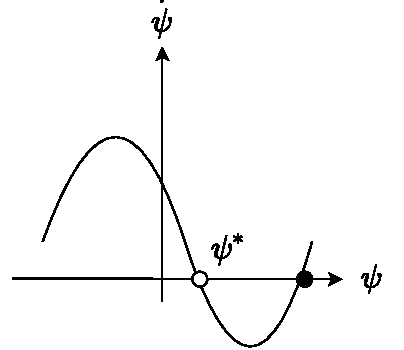
\includegraphics[width=70mm]{images/kuramoto-2.pdf}
\centering
\caption{式\eqref{eq:kuramoto-2body}が安定解を持つ場合.$\delta\psi^\ast$は安定解となる.}
\label{fig:kuramoto-2}
\end{figure}
また,式\eqref{eq:kuramoto-2body}に従う振動子の実効振動数$\langle\dot{\phi}_i\rangle$を以下で定義する.
\begin{align*}
    \langle\dot{\phi}_i\rangle:=\lim_{T\to\infty}\frac{\phi_i(T)-\phi_i(0)}{T}
\end{align*}

式\eqref{eq:kuramoto-2body}を$N$体 ($N\in\mathbb{N}$) に拡張したものは以下のようになる.
\begin{align}
    \label{eq:kuramoto-N}
    \dot{\phi}_i=\omega_i+\frac{K}{N}\sum_{j=1}^N\sin(\phi_i-\phi_j),\ i=1,2,\ldots,N
\end{align}
ここで,$K$は共通の結合強度で,$\omega_i$は振動子$i$の固有振動数とする.
% $g(\omega)=g(-\omega)$となる振動数分布$g(\omega)$に従うとする.

このとき,振動子全体の同期を評価する量として以下で定義されるオーダーパラメータが用いられている.
\begin{align*}
    R\mathrm{e}^{\imag \psi}:=\frac{1}{N}\sum_{j=1}^N\mathrm{e}^{\imag \theta_j}    
\end{align*}
オーダーパラメータは,位相が$[0,2\pi)$に一様に分布しているとき,$R= 0$となる.つまり振動子同士に同期が見られない状態を表す.
一方,振動子全体の位相が一致するとき,$R=1$となる.

式\eqref{eq:kuramoto-N}は,一般の複雑ネットワークにおける位相振動子モデルに拡張できる.
\begin{align*}
    \dot{\phi}_i=\omega_i+\frac{K}{N}\sum_{j=1}^NA_{ij}\sin(\phi_i-\phi_j),\ i=1,2,\ldots,N
\end{align*}
ここで,$A_{ij}$は振動子の接続状況を表す隣接行列$A$の成分で,振動子$i$と振動子$j$の間に枝があれば$1$,そうでなければ$0$である.
一般には,無向グラフ,有向グラフ両方とも考えることがあるが,本論文では無向グラフのみを考えるため,$A$は対称行列となる.
\section{近恒等変換}
本節を書くにあたっては,\cite{james2003}を参考にした.

以下のような周期的な微分方程式を考える.
\begin{align*}
    \dot{y}=\varepsilon f_1(t,y)+\varepsilon^2f_2(t,y)+\cdots
\end{align*}
ただし,$y\in\mathbb{R}^{n-1}$で,$f_j$は$t,y$に関して周期的な関数である.\\
ここで,$x\in\mathbb{R}^{n}$として,$f_j$に対し平均化を行うと
\begin{align*}
    a_0(x)&=[1,0,\ldots,0]^\top\in\mathbb{R}^{n+1}\\
    a_j(x)&=[0,f_j(x)]^\top
\end{align*}
として,
\begin{align*}
    \dot{x}=a(x,\varepsilon)\sim a_0(x)+\varepsilon a_1(x)+\varepsilon^2 a_2(x)+\cdots
\end{align*}
に近似できる.ただしこの展開誤差はコンパクト集合上の任意の$x$で一様収束する.

この式を周期的で$\varepsilon$に依存した変数変換で,自律系に書き換えることを考える.
以下のような変形は条件を満たす,
\begin{align}
    \label{eq:int}
    x=\xi+\sum_{j=1}^k \varepsilon^j s_j(t,\xi)
\end{align}
ここで,$x\in\mathbb{R}^n$,$s_j:\mathbb{R}\times\mathbb{R}^n\to\mathbb{R}^n$は$t$に関して周期的とする,
式\eqref{eq:int}は近恒等変換と呼ばれ,誤差が$O(\varepsilon^k)$の範囲で逆変換が存在する.また,この変換は$x$の周期$x_0$で平均化を行ったことに相当する.

このように,非自律系であっても近恒等変換を用いて自律系に変形することで詳細なふるまいを調べることができ,また周期的な系であっても平均化を行い周期性を保ちながら詳細なふるまいを調べることができる.
\section{ランダムグラフ}
本節を書くにあたっては,\cite{Bollobas2013},\cite{Albert2002}を参考にした.
\subsection{Erdős–Rényi グラフ}
$V=\{1,2,\ldots,n\}$とラベリングされた$n$個の頂点と$N$本の枝を持つランダムグラフ$\Gamma_{n,N}$を考える.
つまり,異なる頂点$i,j\in V,\ i\neq j$との間の枝-全$\binom{n}{2}$本から等しい確率で$N$本選んだものを考える.

$\Gamma_{n,N(n)}$について,$N(n)$によりグラフの連結成分や次数などの性質がどのように変化するかという問題が生じる.
Erdős 及び Rényi は,$N(n)$の増大に伴って巨大な連結成分が出現することを発見し,以下のような結果を得た.

$n$を固定し,$N$を1から$\binom{n}{2}$まで増やしたときに,$\Gamma_{n,N}$は5つの異なる状態を経る.
ただし,漸近的とは,頂点数$n$を十分大きくする操作について述べているとする.
\renewcommand{\labelenumi}{Phase \theenumi}
\begin{enumerate}
    \item 
    $N(n)=O(n)$のとき.\\
    この場合ほとんど確実に$\Gamma_{n,N}$は木である.
    木に含まれる頂点の最大次数が$k$になりうるのは,$N(n)=O(n^{(k-2)/(k-1)})$のときで,そのときの$|\Gamma_{n,N}|$はポアソン分布で,$\Gamma_{n,N}$は正規分布で漸近的に記述される.
    \item
    $N(n)=cn+O(n),\ 0<c<1/2$のとき.\\
    この場合ほとんど確実に,高々1つの閉路しか存在せず,ほとんどの頂点は木に属する.また,頂点数最大の連結成分の頂点数は$|1/\alpha(\log n-5/2\log\log n)|$となる.$(\alpha=2c-1-\log 2c)$
    \item
    $N(n)=cn+O(n),\ c\geq 1/2$のとき.\\
    $N(n)$が$n/2$を超えると最大の連結成分は漸近的に$n^{2/3}$個の頂点を持つが,その構造は複雑でなる.一方,この連結成分以外の連結成分はほとんど確実に木である.
    \item
    $N(n)=cn\log n+O(n\log n),\ c\leq 1/2$のとき.\\
    このときほとんど確実にグラフ全体が連結となる.
    \item
    $N(n)\sim(n\log n)\omega(n)$のとき.\\
    このときグラフ全体が連結なだけでなく全ての頂点の次数が漸近的に等しい.
\end{enumerate}
\renewcommand{\labelenumi}{\theenumi}
\subsection{percolation}
percolation は,ネットワーク全体を貫く (percolate) 道の存在を調べる理論である.
percolation には頂点を固定して枝を確率的に配置する bond percolation と,枝を固定して頂点を確率的に配置する site percolation の2種類が知られている.
いずれの場合も配置確率$p$に対し,主に以下の3つの指標に注目する.
\begin{itemize}
    \item パーコレーション確率$P$\\
        無限に大きいネットワーク$G(V,E)$において,ある頂点がサイズが無限大のクラスター(連結成分)に属する確率である.
        \begin{align*}
            P=P_p(|C|=\infty)=1-\sum_{1<s<\infty}P_p(|C|=s)
        \end{align*} 
        ここで,$P_p(|C|=s)$はある頂点が属するクラスタ$C$のサイズが$s$である確率とする.
        ただし,$|C|/|V|<\infty$となるクラスタ$C$のサイズを$|C|=\infty$と定める.
        このとき,ある臨界確率$p_c$を境に$P$が変化する.
        \begin{align*}
            P
            \begin{cases}
                = 0 & (p<p_c)\\
                > 0 & (p\geq p_c)
            \end{cases}
        \end{align*}
    \item 平均的なクラスタのサイズ$\langle s \rangle$
        \begin{align*}
            \langle s\rangle =E_p(|C|)=\sum_{s=1}^\infty sP_p(|C|=s)
        \end{align*}
        $P>0$のときは$\langle s\rangle$は発散するので,代わりにサイズが有限のクラスタの平均サイズを考える.
        \begin{align*}
            \langle s\rangle^f =E_p(|C|,|C|<\infty)=\sum_{s<\infty} sP_p(|C|=s)            
        \end{align*}
    \item クラスタのサイズ分布$n(s)$
    \begin{align*}
        n(s)=\frac{1}{s}P_p(|C|=s)
    \end{align*}
    ここで,ある頂点がサイズ$s$のクラスタに含まれる確率とは必ずしも一致しないことに注意.
\end{itemize}

ランダムグラフで任意の頂点間に枝を存在しうることは,無限次元の系での bond percolation に対応する.
このことからランダムグラフと percolation のアナロジーを考えることができる.
実際,無限次元系において percolation における臨界確率$p_c$は$p_c\simeq 1/N$となり,Erdős–Rényi グラフの巨大な連結成分が出現する本数と対応する.
\begin{align*}
    \binom{N}{2}p_c\simeq N/2
\end{align*}
同じ問題に取り組む二つの理論が存在することは,互いの理論を相補的に活用することができるため重要視されている.
\section{力学系}
本節を書くにあたっては,\cite{teschlordinary},\cite{Ciesielski+2012+2110+2128}を参考にした.
\subsection{自律系と流れ}
以下のような自律系を考える.
\begin{align}
    \label{eq:autonomous}
    \dot{x}=f(x),\ x(0)=x_0
\end{align}
ただし,$f$は開集合$M\subset \mathbb{R}^n$上で定義された$C^k\ (k\geq 1)$級関数とする.\\
式\eqref{eq:autonomous}の解$\phi:T\subset \mathbb{R}\to M$は積分曲線と呼ばれ,$\phi(0)=x_0$を満たすような積分曲線を$x_0$における積分曲線と呼ぶ.\\
そして,微分方程式の流れを写像として以下のように定義する.
\begin{align*}
    \Phi:W\subset\mathbb{R}\times M\to M,\ (t,x)\mapsto \phi(t,x)
\end{align*}
ここで,$\phi(t,x)$とは$x$における積分曲線のうち,一意性が保証されるような最大の開区間$I_x=(T_-(x),T_+(x))$で定義されたものとする.
\subsection{軌道と不変集合}
$x$における軌道$\gamma(x)$とは以下で定義される.
\begin{align*}
    \gamma(x):=\Phi(I_x\times \{x\})\subset M
\end{align*}
同様に前進軌道,後退軌道が定義される.
\begin{align*}
    \gamma_\pm(x):=\Phi((0,T_\pm (x))\times \{x\})
\end{align*}

また,$\gamma(x)=\{x\}$のとき$x$は$\Phi$の平衡点と呼ぶ.
そして,$\Phi(T,x)=x$なる$T>0$が存在するとき,$x$を周期点と呼び$T$の下限を周期と呼ぶ.
特に,軌道の任意の点が周期点であるとき,その軌道を周期軌道と呼ぶ.

$x\in M$の$\omega_\pm$-極限集合$\omega_\pm(x)$とは,点列$t_n\to \pm\infty$が存在して$\Phi(t_n,x)\to y$となるような点$y\in M$の集合である.\\
集合$U\subset M$が$\sigma$不変 ($\sigma\in\{\pm\}$)とは,以下を満たすこと.
\begin{align*}
    \forall x\in U,\ \gamma_\sigma (x)\subset U
\end{align*}
また,$\pm$どちらでも不変のとき不変であると呼ぶ.\\
集合$U\subset M$が minimal とは,非空で閉かつ不変であるような$M$の部分集合のうち最小のものであることをいう.
\subsection{Poincaré-Bendixsonの定理}
まず,広く知られている$\mathbb{R}^2$上のPoincaré-Bendixsonの定理について述べる.
\begin{theorem}
    以下の自律系について,解が一意に与えられ任意の$t\in\mathbb{R}$で定義されるとする.
    \begin{align}
        \dot{x}=f(x),\ x\in M\subset \mathbb{R}^2,\ f\in C^1(M,\mathbb{R}^2),\ M:\mathrm{open}         \label{eq:automonous-poincare}
    \end{align}
    $p\in M$の前進軌道$\gamma_+(p)$が連結な有界閉集合で,$\omega$極限集合$\omega(p)$が一つも平衡点を持たないと仮定する.
    このとき,$\omega(p)$は周期軌道で$p$が周期点であるか,$\gamma_+(p)$がLimit Cycleに収束するかのどちらかである.
    \label{theorem:poincare}
\end{theorem}
この定理により閉軌道の存在を示すことができるため,具体的に周期解を求めることが難しい非線形力学系の分野で重要な定理となっている.

一方,$\mathbb{R}^2$と同じ2次元平面であっても,トーラス$\mathbb{T}^2$では異なるふるまいを示す.
Schwartzは定理\ref{theorem:poincare}を任意の二次元多様体に拡張した\cite{Schwartz1963ErrataAG}.
\begin{theorem}
    \label{thm:poiben-gen}
    $C^2$級のコンパクトで連結な二次元多様体$X$で定義された自律系 (式\eqref{eq:automonous-poincare}) が流れを与えるとする.
    集合$M\subset X$がminimalならば,$M$は次のうちのどれか一つである.
    \begin{enumerate}
        \item 平衡点からなる一元集合
        \item 単純かつ閉で$\mathbb{S}^1$に同相な軌道
        \item $\mathbb{T}^2$に同相な$X$全体
    \end{enumerate}
\end{theorem}
\subsection{準周期軌道}
準周期軌道とは,周期的ではあるもののほぼ周期的でないくらい周期が長いような軌道のことであり,
惑星の軌道や周期運動に摂動を加えた系でよく見られる.

準周期性は,厳密には以下のように定義される\cite{Broer1996}.\\
不変な$n$トーラス$\mathbb{T}^n$の多様体$M$上の滑らかなベクトル場$X$を考える.\\
制限$X|_T$を$\dot{x}_i=\omega_i,\ i=1,2,\ldots ,n$に写す微分同相写像$T\to \mathbb{T}^n$が存在するとき,$T$上の$X$が parallel な流れを誘導するという.
そして,$\omega=(\omega_1,\omega_2,\ldots,\omega_n)$を$T$上の流れの振動数という.\\
振動数$\omega$が rationally independent, i.e., $\forall k\in\mathbb{Z}^n\setminus \{0\},\ \sum_{i=1}^n\omega_ik_i\neq 0$のとき,振動数$\omega$をもつ parallel な$T$上の流れは準周期的もしくは非調和的と呼ぶ.

例えば,$\mathbb{T}^2$上の流れ$\dot{x}_1=\omega_1,\ \dot{x}_2=\omega_2$が準周期的である必要十分条件は振動数の比$\omega_1/\omega_2$が無理数であることである.

準周期的な流れによる軌道は,流れが定義された空間全体を密に満たす.しかしながら,初期値に鋭敏に依存しないためカオスとは区別される.
\end{document}